\documentclass[11pt, oneside]{article}   	% use "amsart" instead of "article" for AMSLaTeX format
\usepackage{geometry}                		% See geometry.pdf to learn the layout options. There are lots.a 
\geometry{letterpaper}                   		% ... or a4paper or a5paper or ... 
%\geometry{landscape}                		% Activate for for rotated page geometry
%\usepackage[parfill]{parskip}    		% Activate to begin paragraphs with an empty line rather than an indent
\usepackage{graphicx}				% Use pdf, png, jpg, or eps� with pdflatex; use eps in DVI mode
								% TeX will automatically convert eps --> pdf in pdflatex		
\usepackage{amssymb}
\usepackage{amsmath}
\usepackage{parskip}
\usepackage{color}
\usepackage{hyperref}

\title{Karkhar Video 27}
%\author{The Author}
%\section{}
%\subsection*{}
\date{}							% Activate to display a given date or no date

\graphicspath{{/Users/telliott_admin/Dropbox/Tex/png/}}
% \begin{center} 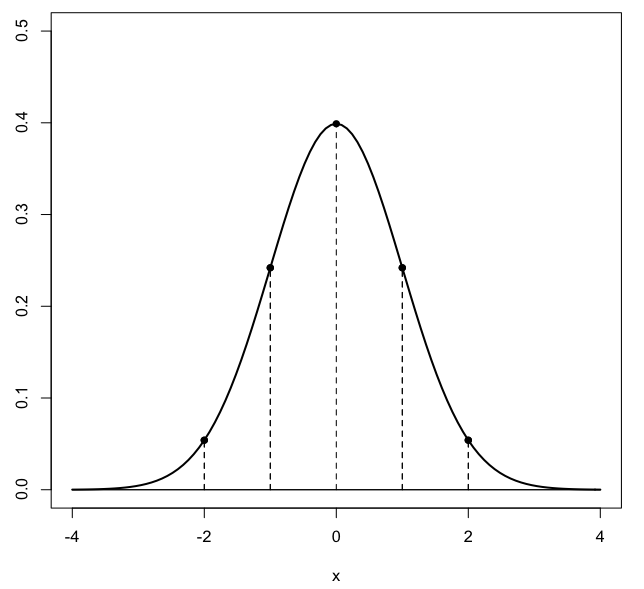
\includegraphics [scale=0.4] {gauss3.png} \end{center}
\begin{document}
\maketitle
\Large
Karkhar gives this problem
\[ \int_0^{2\pi} \frac{1}{2 + \cos \theta} \ d \theta \]
Before we start I'd just point out that the equation for an ellipse in polar coordinates (with one focus at the origin) is
\[ r = \frac{b^2}{a - c \cos \theta} \]
If we neglect the minus sign (which just flips the orientation along the $x$-axis), let $a=2$ and $c=1$ and
\[ b^2 = a^2 - c^2 = 3 \]
rewrite
\[ \int_0^{2\pi} \frac{3}{2 + \cos \theta} \ d \theta \]
What this looks like to me is the integral of $r \ d \theta$ around an ellipse with $a = 2$ and $b = \sqrt{3}$.  This would be $r d \theta$ added up over the perimeter of that ellipse, i.e. the area.

Go back to the given problem.  Let
\[ z = e^{i\theta} \]
\[ dz = i z \ d \theta \]
\[ \cos \theta = \frac{1}{2}(e^{i\theta} + e^{-i \theta} ) \]
Use this result, but go back to $z$:
\[ \int_{|z|=1} \frac{1}{2 + (1/2)(z + 1/z)} \ \frac{1}{iz} \ dz \]
\[ = \frac{1}{i}  \int_{|z|=1} \frac{1}{2z + (1/2)(z^2 + 1)} \ dz \]
\[ = \frac{2}{i}  \int_{|z|=1} \frac{1}{z^2 + 4z + 1} \ dz \]
The roots of the denominator are $-2 \pm \ \sqrt{3}$.  One of these roots ($-2 + \sqrt{3}$) lies within our contour, which is just the unit circle.

Carry out partial fractions:
\[ \frac{1}{z^2 + 4z + 1} = \frac{A}{z - (-2 + \sqrt{3})} + \frac{B}{z - (-2 - \sqrt{3})} \]
\[ Az + A2 + A \sqrt{3} + Bz + B2 - B \sqrt{3} = 1 \]
Hence $A = -B$ and
\[ A2 + A \sqrt{3} -A2 + A \sqrt{3} = 1 \]
\[ 2A \sqrt{3} = 1 \]
\[ A = \frac{1}{2 \sqrt{3}} \]
The term we want is the one with $z_0 = (-2 + \sqrt{3})$ and that has coefficient $A$.  Hence the value is
\[ 2 \pi i \ (\frac{1}{2 \sqrt{3}}) = \frac{\pi i}{\sqrt{3}} \]
Pick up the leading factor of $2/i$ and obtain $2 \pi / \sqrt{3}$.

Going back to the argument about the ellipse at the beginning, multiplied by $3$ this gives $2 \sqrt{3} \pi$.  This is exactly the area of an ellipse with $a = 2$ and $b = \sqrt{3}$.

\end{document}  